\subsection{Measurement-Based Quantum Computation (MBQC)}

Measurement-Based Quantum Computation (MBQC) is an alternative model of
quantum computation where the computation is driven by single-qubit
measurements on a pre-prepared entangled resource state \cite{}. A canonical example of
such a resource state is the \emph{cluster state} is shown in Figures \ref{fig:graph}. The computation proceeds as follows:

%or its universal variant, the
%\emph{brickwork state}, which are shown in Figures \ref{fig:graph} and \ref{fig:brick}. The computation proceeds as follows:

\begin{enumerate}
  \item Prepare a highly entangled resource state $\ket{G}$ associated to a
        graph $G=(V,E)$.
  \item For each vertex $v \in V$, perform a single-qubit measurement in the
        basis
        \[
        \{ \, \ket{+_{\delta_v}}, \ket{-_{\delta_v}} \, \}, 
        \qquad \ket{\pm_{\delta}} = \tfrac{1}{\sqrt{2}}(\ket{0} \pm e^{i\delta}\ket{1}),
        \]
        where $\delta_v$ is the measurement angle.
  \item Later measurement angles $\delta_v$ are adapted according to previous
        measurement outcomes (classical feed-forward).
\end{enumerate}



\begin{figure}
    \centering
    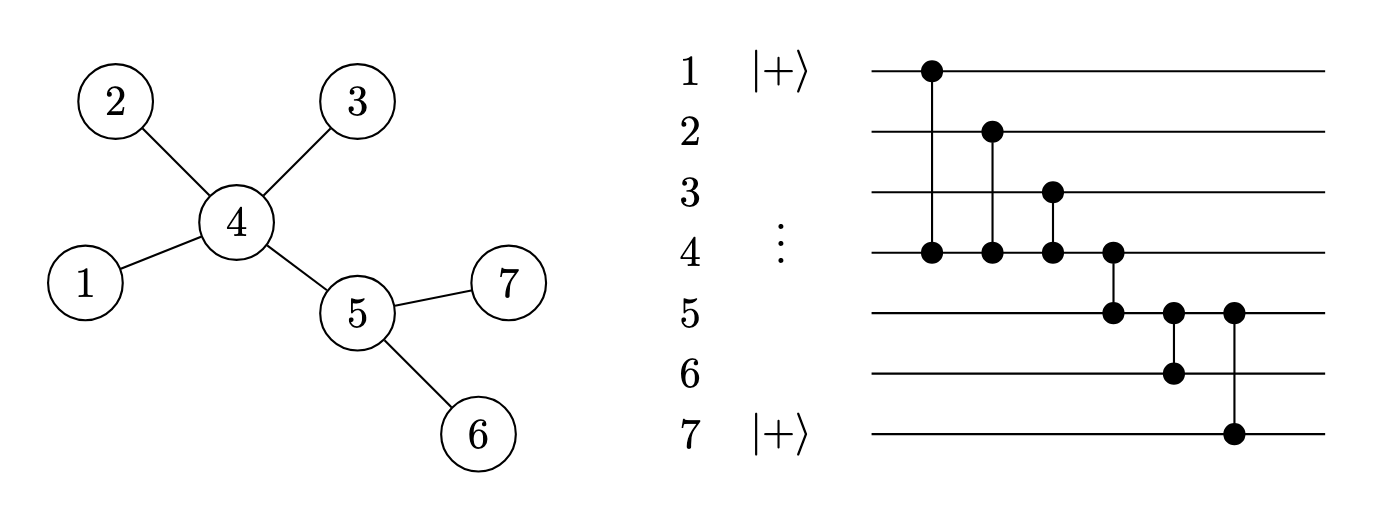
\includegraphics[width=0.5\linewidth]{graph.png}
    \caption{Translation of a graph state (left) into a circuit (right). Vertices correspond to qubits prepared in $\ket{+}$ and CZ gates between qubits correspond to vertices that share an edge in the graph.}
    \label{fig:graph}
\end{figure}


Universality arises because any quantum circuit can be implemented as a
sequence of such measurements on the brickwork state, with the adaptivity
providing the needed conditional operations.  In this paper, we work on arbitrary graph state, beyond the brickwork state.
% \begin{comment}
% \begin{figure}
%     \centering
%     \includegraphics[width=0.5\linewidth]{brick.png}
%     \caption{CNOT gate on the brickwork state. All measurements are in the XY plane. Squares indicate output nodes.}
%     \label{fig:brick}
% \end{figure}
% \end{comment}
\subsection{Blind Quantum Computation (BQC)}

Blind Quantum Computation (BQC) addresses the scenario where a client (with limited quantum capability) wishes to delegate a computation to a quantum server without revealing the computation itself \cite{}. Blindness means that the server learns nothing about the client’s input, output, or algorithm, beyond upper bounds on size parameters such as circuit width and depth.

The MBQC framework naturally lends itself to blindness: the client can prepare
randomized single-qubit states
\[
\ket{+_{\theta}} = \tfrac{1}{\sqrt{2}}(\ket{0} + e^{i\theta}\ket{1}),
\qquad \theta \in \Theta = \{0,\tfrac{\pi}{4},\dots, \tfrac{7\pi}{4}\},
\]
and send them to the server. Since the phases are randomized, the server cannot
distinguish whether a given qubit will serve as a trap, a dummy, or a
computational qubit.

\subsection{Universal Blind Quantum Computation (UBQC)}

Universal Blind Quantum Computation (UBQC) is a protocol introduced to achieve
perfect blindness within the MBQC model \cite{}. The idea is:

\begin{itemize}
  \item The client prepares single-qubit states $\ket{+_{\theta_v}}$ for
        randomly chosen $\theta_v \in \Theta$ and sends them to the server.
  \item The server entangles these qubits according to the graph state via
        $CZ$ gates, forming a universal resource state.
  \item To instruct the server on how to measure qubit $v$, the client computes
        a disguised measurement angle
        \[
        \delta_v = \phi_v + \theta_v + r_v \pi,
        \]
        where $\phi_v$ is the intended computation angle and $r_v \in \{0,1\}$
        is a secret random bit.
  \item The server measures in the $\{ \ket{\pm_{\delta_v}} \}$ basis and
        reports the outcome to the client.
\end{itemize}

Because of the random offsets $\theta_v$ and $r_v$, the server obtains no
information about $\phi_v$ (the true computational angles). Yet, the client can
decrypt the measurement outcomes and recover the intended computation.

\paragraph{Properties.}
\begin{itemize}
  \item \textbf{Correctness:} UBQC reproduces the same distribution of outcomes
        as MBQC on the intended circuit.
  \item \textbf{Blindness:} The distribution of states and instructions sent to
        the server is independent of the actual computation. The only leakage
        is the circuit size (width $W$ and depth $D$).
\end{itemize}

\paragraph{Role in Verification.}
UBQC provides a perfect blindness layer that can be extended with traps to
achieve \emph{verifiable blind quantum computation} (VBQC). In trap-based VBQC
protocols, the client intersperses trap qubits among computational qubits in
such a way that deviations by the server are caught with high probability.
Thus, MBQC and UBQC are the foundation upon which robust VBQC and further
extensions such as ACES are built.

\subsection{Robust VBQC}
Trap-based protocols extend UBQC by adding verifiability. The client hides
special trap qubits among the computation, which are deterministically
prepared, and whose outcomes are known in advance. Any deviation by the server
has a probability of being detected.

\subsubsection{Protocol 1 (Noise-Robust VBQC for BQP Computations)}
\textbf{Client's Inputs:} 
\begin{itemize}
  \item A circuit $C$ implemented on a graph state of $G(V, E)$.
  \item $n \in 2\mathbb{N}$ rounds for the protocol.
\end{itemize}

\noindent
\textbf{Round Delegation:}
\begin{enumerate}
  \item The client randomly partitions $[n]$ into computation rounds $C$ and
        test rounds $T$, with $|C|=|T|=n/2$.
  \item For $j \in T$, the client chooses a random color $V_j \in \{V_1,V_2\}$,
        and delegates a UBQC trap round.
  \item For $j \in C$, the client delegates computation $C$ using UBQC.
\end{enumerate}

\noindent
\textbf{Acceptance Criterion:}
\begin{itemize}
  \item For each $j \in T$, check all trap outputs decrypt to the expected
        $|+\rangle$ measurement.
  \item Let $t_{\mathrm{fail}}$ be the number of failed trap rounds.
\end{itemize}

This protocol ensures the correctness, security, and robustness \cite{}.

% \begin{comment}



% \noindent
% \textbf{Result Computation:}
% \[
% \text{If } t_{\mathrm{fail}} < w (\text{Some threshold value}), \quad
% x = \text{majority vote over outputs of computation rounds}, \quad
% \text{Output } (x,\mathrm{Accept}).
% \]
% Otherwise, output $(\perp,\mathrm{Reject})$.

% \subsection*{Theorem 1}
% Let $C$ be a set of BQP instances with error upper bounded by $c$. For $n \in
% 2\mathbb{N}$ and threshold $w/t$ fixed with $0 < w/t < \tfrac{1}{2}
% \tfrac{1-2c}{2-2c}$, Protocol 1 $\epsilon$-securely constructs the verified blind
% resource in the Abstract Cryptography framework with $\epsilon$ negligible in $n$.

% \subsection*{Correctness}
% Using Hoeffding’s inequality:
% \[
% \Pr[\text{Return No} \mid \text{Yes instance}] 
%   \leq \exp\left(-2 \left(\tfrac{1}{2} - c\right)^2 d\right),
% \]
% which vanishes exponentially in the number of computation rounds $d = n/2$.

% \subsection*{Security}
% The distinguishing advantage of any malicious server reduces to the probability
% of both flipping the majority of computation rounds and avoiding trap detection.
% The blindness of UBQC ensures that deviations can be modeled as Pauli attacks,
% with $Y$ or $Z$ anticommutes on trap stabilizers detected with probability at
% least $1/2$. Security error is bounded by
% \[
% \epsilon_{\mathrm{sec}} \leq 
% \exp\left(-\frac{\phi^2}{8}\Big(\frac{1-2c}{2-2c} - \phi\Big)n\right) 
% + \exp\left(-\Big(\tfrac{1}{2}-2c+\tfrac{\phi}{2}\Big)\phi'^2 n\right),
% \]
% for $d=t=n/2$, $0 < \phi < \tfrac{1-2c}{4-4c}$, and $\phi'=\frac{\phi(1-c)^2}{1+\phi(1-c)}$.

% \subsection*{Robustness}
% If the noise level $p_{\mathrm{err}}$ satisfies $p_{\mathrm{err}} \leq 2(\tfrac{w}{t} - \phi'')$
% for some $\phi''>0$, then
% \[
% \Pr[\mathrm{Reject}] \leq \exp(-\phi''^2 n).
% \]
% Thus the robust-correctness error is
% \[
% \epsilon_{\mathrm{rob}} \leq \epsilon_{\mathrm{sec}} + \exp(-\phi''^2 n),
% \]
% guaranteeing acceptance under bounded noise.

% % ==========================
% % ACES (Averaged Circuit Eigenvalue Sampling)
% % ==========================
% \end{comment}
% \begin{comment}
    

% \section*{Global Noise Assumptions}
% \subsection*{Single Global Parameter}
% Suppose that after each $CZ$ operation, both qubits are affected by the same
% single-qubit depolarizing channel with a uniform parameter $p_{\mathrm{err}}$
% independent of their identity. In the Pauli transfer picture, such a channel
% shrinks non-identity Paulis by a factor $\alpha = 1-\tfrac{4}{3}p_{\mathrm{err}}$.

% For any trap stabilizer $K_v$, the effect of noise under a given ordering is
% captured by a multiplicative factor $\alpha^w$, where $w$ counts how many times
% the evolving Pauli associated with $K_v$ overlaps with a noisy support. The
% resulting failure probability is
% \begin{equation}
% p_{\mathrm{fail}} = \frac{1}{2}\bigl(1-\alpha^w\bigr).
% \end{equation}
% Thus, estimation of $\alpha$ only requires a single equation, since all traps
% collapse to the same functional form. A practical estimator is
% \begin{equation}
% \hat{\alpha} = (1-2p_{\mathrm{fail}})^{1/w}.
% \end{equation}
% The exponent $w$ can be determined from the structure of the graph state and
% the chosen ordering.

% \subsection*{Two-Qubit Depolarizing Noise}
% Consider instead a uniform two-qubit depolarizing channel applied after each
% $CZ$ gate. In this model, each non-identity two-qubit Pauli operator is shrunk
% by the same factor $\alpha$. Hence, the success-failure bias of a trap satisfies
% \begin{equation}
% 1-2p_{\mathrm{fail}} = \alpha^m,
% \end{equation}
% where $m$ is the number of noisy $CZ$ applications that touch the support of the
% stabilizer. The corresponding estimator is
% \begin{equation}
% \hat{\alpha} = (1-2p_{\mathrm{fail}})^{1/m}.
% \end{equation}

% In terms of the physical depolarizing probability $p$, we have the relation
% \begin{equation}
% p = \frac{15}{16}(1-\alpha).
% \end{equation}
% This is because the two-qubit depolarizing channel mixes uniformly among the
% $15$ non-identity Paulis on two qubits. Thus, all trap data can be combined to
% yield a global estimate of $p$ with small statistical variance.

% \end{comment}

\subsection{ACES}
Averaged Circuit Eigenvalue Sampling (ACES) provides a method to characterize
Pauli noise parameters affecting Clifford circuits \cite{}.

\subsubsection{General Principle}
For a Clifford circuit $C = C_n \cdots C_0$, noisy implementation
$\tilde{C}_k$, \(\ k \in \{0,\ldots n\}\) are Clifford gates and Pauli operator $P$, Pauli noise yields
\[
\Lambda(C,P) \, C[P] = \tilde{C}[P],
\]
where $\Lambda(C,P)$ are generalized eigenvalues encoding the noise parameters that depend on \(P\), and on the ordered sequence of Clifford gates \(C = C_n, \ldots C_0\).



% \begin{comment}

% ACES offers a template methodology for learning Pauli-noise model parameters affecting Clifford operations of a quantum circuit. It works by recognizing that Pauli operators are eigenvectors of such noise models and that, because Clifford gates map Paulis to Paulis, after a sequence of noisy Clifford gates, Pauli operators obey a generalized eigenvalue equation of the form
% \begin{equation}
% 	\Lambda(C_n, \ldots C_0,  P) C_n \circ \ldots C_0 [P] = \tilde C_n \circ \ldots \tilde C_0 [P],
% \end{equation}
% where \(P\) is a Pauli operator, \(C_k, \ k \in \{0,\ldots n\}\) are Clifford gates and \(\tilde C_k\) their respective noisy versions, for a Pauli noise model. \(\Lambda\) are the generalized eigenvalues that depend on \(P\), and on the ordered sequence of Clifford gates \(\mathcal C = C_n, \ldots C_0\).
% \end{comment}
The general idea of ACES is to (i) vary the sequence \(C\) of Clifford gates and the chosen \(P\)s to get several relationships between the \(\Lambda\)s and the noise parameters;
(ii) to estimate each \(\Lambda\) by preparing an eigenstate of \(P\) and measuring the Pauli observable \(C_n \circ \ldots C_0[P]\) at the output of the circuit;  and (iii) recover the values of the noise parameters by inverting the system of equations obtained at the previous step. 

%For more details of noise estimation of brickwork state, please see Appendix \ref{app1}. In this paper, we exhibit the noise estimation beyond brickwork state, i.e., arbitrary graph state, which is discussed next.


%\subsection*{Generic Graph States}


